\begin{minipage}[t]{180mm}
\fcolorbox{black}{white}{
\begin{minipage}[b]{30mm}

\includegraphics[width=0.5\linewidth]{unflogo.pdf}
\end{minipage}
\begin{minipage}[b]{100mm}
\Huge \textbf{UNF NEWZ} \\
\Large -- Søvn og retsstavning er overvurderet! 
\end{minipage}
\begin{minipage}[b]{50mm}
\Large Onsdag 17.07.2015 \\
\normalsize Redigeret i \LaTeX\ af \\ SOM, MGS, MMN, SABH
\end{minipage}
}
\end{minipage}



\begin{minipage}[b]{0.95\linewidth}
\begin{minipage}[t]{0.47\textwidth}
\vspace{3mm}
\section*{Læserbrev: Skandale}
Kaere alle deltagere og arrangoerer paa dette aars camp!

Det er med stor sorg, at vi maa meddele, at grundet kommunikationsproblemer med campens oeverste ledelse, at vi ikke vil kunne deltage i dette aars camp. 
Det forholder sig saadan, st vi i oejeblikket befinder os i Sultan Hamengkoeboewono X's by, der i daglig tale kaldes Arhusaan paa det lokale sprog Bahasa Indonesia. 
Vi har beklagevis derfor faaet forvekslet denne by med Aarhus. Vi burde maaske have anet uraad, da Himmelbjerget her ligger nord for byen og eftersigende skulle vaere en meget aktiv vulkan! Men Jylland er jo et meget fremmed land for os Koebenhavnere/Fynboere, saa man ved jo aldrig helt, hvad man kan vente sig? Det er jo et udbredt faktum, at Jylland er lidt af et land i sig selv!
Vi maa derfor oenske jer alle en god camp og fortsat god sommer!

Mvh.Ann-Sofie (eks-Fysikcampkoordinator) og Sebastian (eks-Matematikcampkoordinator)

En kort vejudsigt her til sidst: meget varmt og solrigt, dog lidt skyer hen paa dagen og med lidt held en svag koelende brise.

PS. Husk ikke at spise om dagen i loebet af Ramadahen!

\section*{Tvunget i eksil}



\end{minipage}
\hfill\begin{minipage}[t]{0.47\textwidth}

\vspace{1mm}
\tikzstyle{mybox} = [draw=white, fill=blue!20, very thick,
    rectangle, rounded corners, inner sep=10pt, inner ysep=20pt]
\tikzstyle{fancytitle} =[fill=red, text=white]

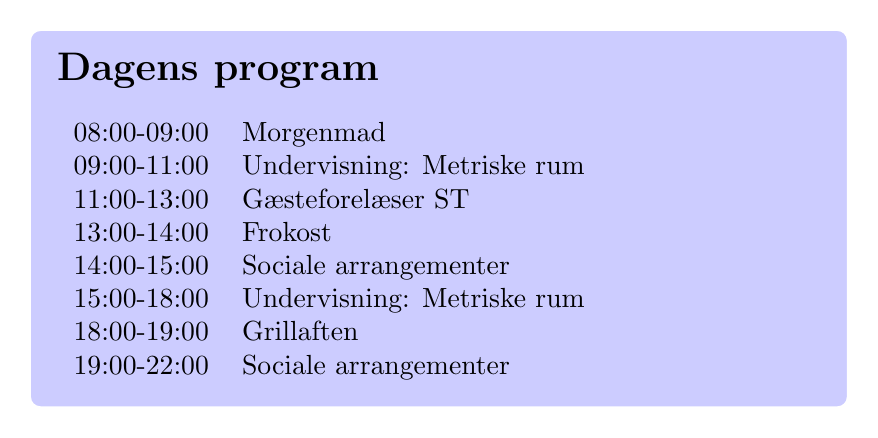
\begin{tikzpicture}
\node [mybox] (box){%
\begin{minipage}{0.80\textwidth}
\vspace{-4mm}\section*{Dagens program}
\begin{tabular}{ll}
08:00-09:00 & Morgenmad \\
09:00-11:00 & Undervisning: Metriske rum \\
11:00-13:00 & Gæsteforelæser ST \\
13:00-14:00 & Frokost \\
14:00-15:00 & Sociale arrangementer \\
15:00-18:00 & Undervisning: Metriske rum \\
18:00-19:00 & Grillaften \\
19:00-22:00 & Sociale arrangementer
\end{tabular}
\vspace{-4mm}
\end{minipage}
};
\end{tikzpicture}%
\vspace{2mm}
\section*{Brandbelæring}
Vi er blevet gjort opmærksom på, at den brandbelæring deltagerne modtog søndag ikke var fyldestgørende, så derfor kommer der her en mere udførlig brandbelæring. I tilfælde af mindre brand på instituttet skal Auditorium E forlades gennem nødudgangene og alle skal samle sig på græsplanen. Såfremt branden viser sig at være større, vil også denne plane skulle forlades, og vi samles i stedet på pladsen overfor Statsbiblioteket. I fald af at branden vokser sig større, specielt hvis den skulle gribe over til kemi, er dette sted på randen af Universitetsparken dog lidt for tæt på, og vi vil derfor i stedet samle os på Østbanetorvet, hvilket ved endnu større brande, for eksempel i Fysiks accelerator også gør det lettere at forlade byen ad sø- eller landvejen. Skulle branden skyldes krigeriske handlinger, specielt med fissionsvåben, anbefales det at Jylland forlades omgående, til dette formål er der flere mulige router. 


\end{minipage}
\end{minipage}
